We solve the objective function of the TV and box constrained FWI using PDS, which is expressed by the following equation:
\begin{equation} \label{eq:FWIObjectiveWithTVConstraint} \FWIObjectiveWithTVConstraint \end{equation}
where $\alpha \in \realNumber$ is the upper bound of the $l_{1,2}$ norm, and $a, b \in \realNumber$ are the lower and upper bounds of the velocity model, respectively.

\begin{figure*}[htbp]
    \centering
    \begin{tabular}{m{68mm} m{70mm} m{10mm}}
        % First row: Image 1, 2, and vertically spanning Image 5
        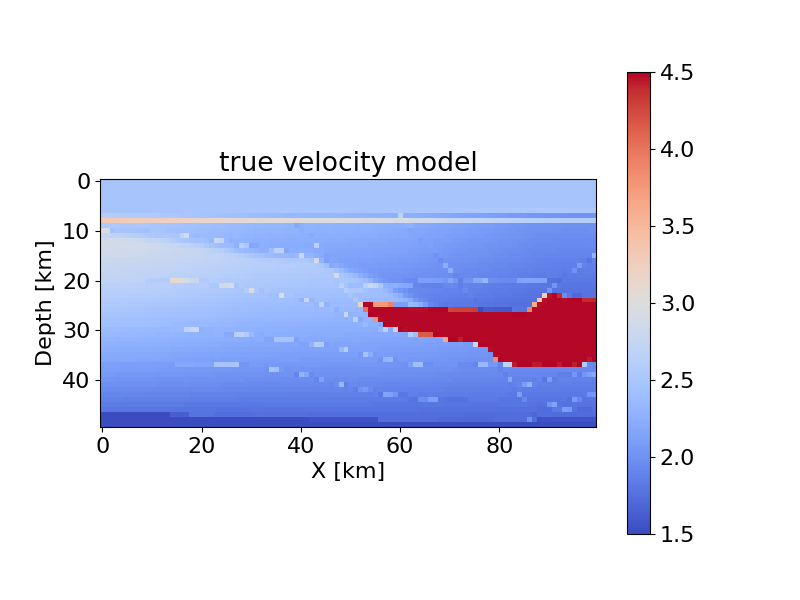
\includegraphics[width=70mm]{public/true} &
        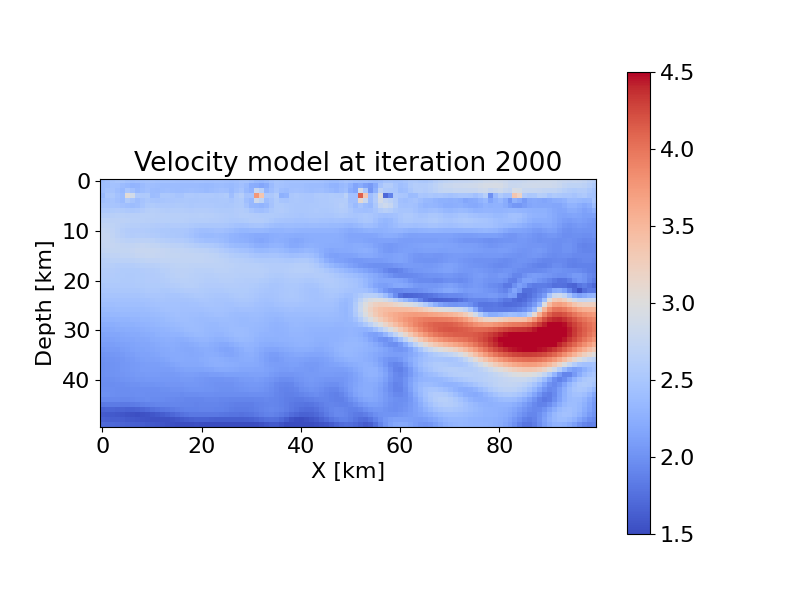
\includegraphics[width=70mm]{public/gradient} &
        \multirow[t]{2}{*}{\raisebox{-46mm}{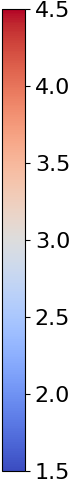
\includegraphics[height=60mm]{public/color-bar}}} \\
        % Second row: Image 3 and 4
        
\includegraphics[width=70mm]{public/initial} &
        
\includegraphics[width=70mm]{public/pds} &
    \end{tabular}
    \caption{LT: background truth model, RT: initial model, LB: gradient method, RB: PDS method}
\end{figure*}



To apply PDS, the constraints are integrated into the objective function as indicator functions:
\begin{equation} \label{eq:FWIObjectiveWithTVConstraintWithIndicatorFunction} \FWIObjectiveWithTVConstraintWithIndicatorFunction \end{equation}
As mentioned in section~\ref{subsec:mathematical-tools}, $\iota_{\LOneTwoNorm{\cdot} \le \alpha}$ and $\iota_{[a,b]^N}$ can be computed efficiently\eqref{eq:ProximityOperatorForL1Ball}\eqref{eq:ProximityOperatorForL12Ball}.
The gradient ${\nabla E(\cdot)}$ can be computed using the adjoint-state method~\cite{FWI-gradient}.

$f$, $g$ and $h$ in \eqref{eq:PDSPrimalEq} correspond to $E$, $\iota_{[a,b]^N}$ and $\iota_{\LOneTwoNorm{\cdot} \le \alpha}$, respectively.
Therefore, the iterative procedures are as follows:
\begin{equation} \label{eq:FWIWithPDS} \FWIWithPDS \notag \end{equation}

